%**************************************************************
\section{Architetture a confronto}
\label{sec:architetture-confronto}

Prima di procedere con la progettazione delle componenti in dettaglio e della vista si sono analizzati più \gls{designpatterng} architetturali per capire quale fosse il più adeguato per lo scopo.\\
La scelta è stata influenzata da fattori come la facilità di implementazione, la facilità di adattamento a \emph{Flutter} e di conseguenza la disponibilità di esempi.\\
Mentre per sviluppare un'applicazione nativa in Android è consigliato usare l'architettura Model View Presenter e in \emph{Qt} quella Model View (una versione modificata di Model View Controller), per Flutter non c'è ancora una \gls{bestpracticeg} diffusa.

%**************************************************************
\subsection{Model View Controller}
\label{subsec:model-view-controller}

Il \emph{Model View Controller (MVC)} è un tipo di architettura molto famosa e molto implementata, ma spesso in maniera errata.\\
Permette di avere, nel proprio sistema, tre componenti che hanno compiti distinti (e lo stesso vale per le altre architetture).\\
In MVC:
\begin{itemize}
    \item il \emph{Model} rappresenta il modello dei dati, ovvero tutto ciò che implementa la \emph{business logic}, comprese le operazioni sui dati (lettura e scrittura da supporti di persistenza e da remoto). Quando viene aggiornato, si occupa di notificare la \emph{View} (tramite il \gls{designpatterng} Observer\footnote{Per maggiori informazioni su Observer, consultare alla sotto-sezione "\hyperref[subsec:observer-provider-changenotifier]{Il design pattern Observer: Provider, ChangeNotifier e Consumer}".});
    \item la \emph{View} rappresenta la parte di \emph{presentation logic}, ovvero ciò che permette di interagire con l'utente. Gli input dell'utente vengono catturati e inoltrati al \emph{Controller};
    \item il \emph{Controller} rappresenta la parte di \emph{application logic} poiché seleziona la \emph{View} corretta in base all'input e inoltra i dati dell'interazione dell'utente al \emph{Model}.
\end{itemize}
Questa architettura è facilmente applicabile in \emph{Flutter}, poiché la vista è correttamente separata dal modello e si gestisce autonomamente il proprio aggiornamento (ad eccezione della selezione che la fa il \emph{Controller}).\\
Sebbene siano separati, la dipendenza della vista dal modello non li rende completamente separati per cui il modello, dovendo fornire metodi per le richieste provenienti dalla vista, dovrebbe già preparare i dati in un formato adeguato, rendendolo più complesso.

\begin{figure}[!h]
    \centering 
    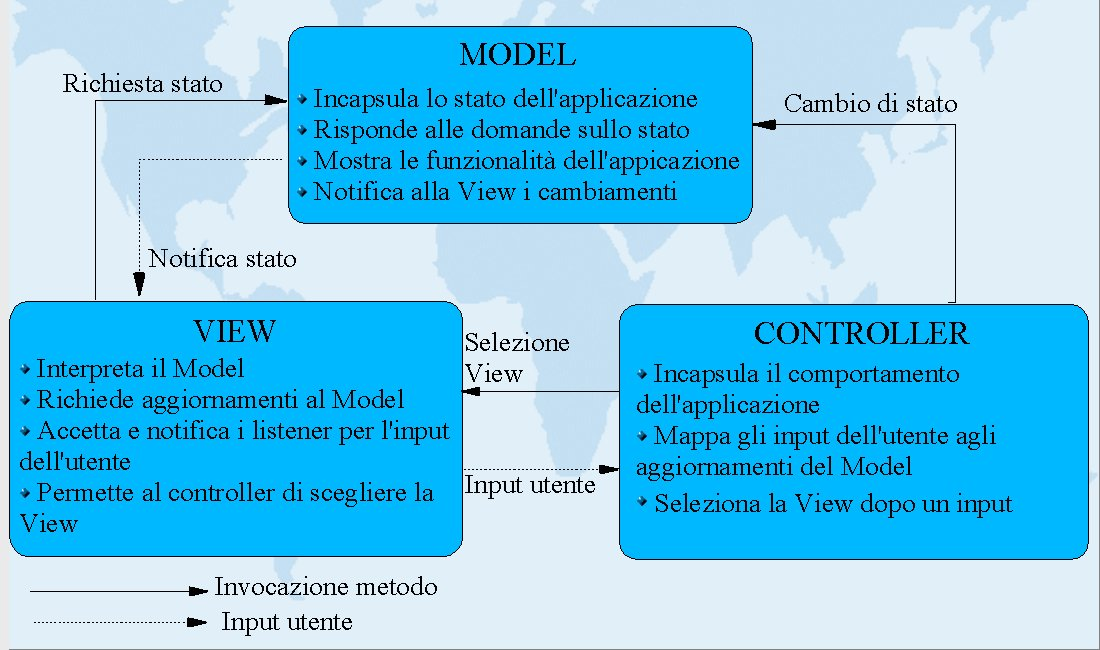
\includegraphics[width=0.9\columnwidth]{capitolo-6/architetture-confrontro/mvc} 
    \caption{Diagramma dell'architettura MVC (da \cite{site:mvc})}
\end{figure}

%**************************************************************
\subsection{Model View Presenter}
\label{subsec:model-view-presenter}

Il \emph{Model View Presenter (MVP)} è invece un'architettura in cui il modello e la vista sono due entità completamente separate e fra di loro sconosciute.\\
Più in dettaglio:
\begin{itemize}
    \item il \emph{Model} rappresenta il modello dei dati, ovvero tutto ciò che implementa la \emph{business logic}, comprese le operazioni sui dati (lettura e scrittura da supporti di persistenza e da remoto). Non notifica la \emph{View} in caso di aggiornamento, ma chiama il \emph{Presenter};
    \item la \emph{View} rappresenta la pura interfaccia di visualizzazione per l'utente (è passiva) oppure può anche contattare il \emph{Presenter} in caso di eventi, in base all'implementazione;
    \item il \emph{Presenter} agisce da "Man in the middle" poiché fa da passacarte fra la \emph{View} e il \emph{Model}. A meno che non sia la \emph{View} stessa a chiamarlo, resta in ascolto di notifiche da parte di entrambi e aggiorna lo stato dell'applicazione o della vista in base alle necessità.
\end{itemize}
Con questo approccio c'è una separazione dei compiti importante ma è richiesto che il \emph{Presenter} si occupi dell'aggiornamento della vista, rendendolo poco adatto a \emph{Flutter}.

\begin{figure}[!h]
    \centering 
    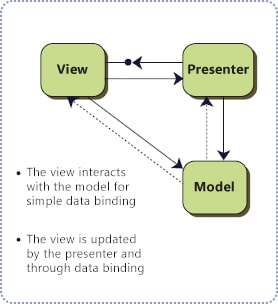
\includegraphics[width=0.5\columnwidth]{capitolo-6/architetture-confrontro/mvp} 
    \caption{Diagramma dell'architettura MVP (da \cite{site:mvp})}
\end{figure}

%**************************************************************
\subsection{Model View ViewModel}
\label{subsec:model-view-viewmodel}

Il \emph{Model View ViewModel (MVVM)} è un'architettura che consente di separare il modello e la vista utilizzando un doppio Observer.\\
Più specificatamente:
\begin{itemize}
    \item il \emph{Model} è il medesimo dell'architettura MVP;
    \item la \emph{View} è la medesima dell'architettura MVC, ma chiaramente in caso di input viene contattato un \emph{ViewModel} e non un \emph{Controller};
    \item il \emph{ViewModel} è il "modello della vista", ovvero il \emph{Model} accinge solo da questo, che accinge a sua volta solo dal \emph{Model}.
\end{itemize}
In MVVM, la \emph{View} è spesso implementata dichiarativamente (e questo è un punto a favore per \emph{Flutter}).\\
Come è stato detto, la \emph{View} può sfruttare il proprio \emph{ViewModel} per ottenere i dati da visualizzare e il \emph{ViewModel} a sua volta utilizza il proprio \emph{Model}.
Essendo implementato il \gls{designpatterng} Observer, quando il \emph{Model} e il \emph{ViewModel} hanno nuovi dati notificano i propri listener (che sono rispettivamente delle \emph{View} e dei \emph{ViewModel}), senza sapere chi è il destinatario.\\

\begin{figure}[!h]
    \centering 
    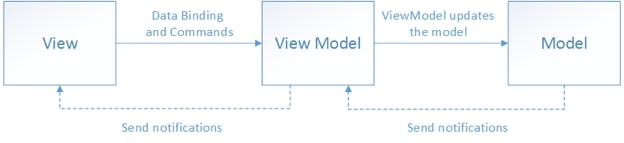
\includegraphics[width=0.7\columnwidth]{capitolo-6/architetture-confrontro/mvvm} 
    \caption{Diagramma dell'architettura MVVM (da \cite{site:mvvm})}
\end{figure}

%**************************************************************
\subsection{Clean Architecture}
\label{subsec:clean-architecture}

La \emph{Clean Architecture} si differenza molto dalle altre tre perché si concentra su una cosa fondamentale: le \textbf{dipendenze} e come \textbf{minimizzarle}.\\
In questo tipo di architettura le dipendenze vanno solo in un verso, che nel diagramma dell'architettura corrisponde dall'esterno all'interno degli strati del cerchio.\\
Più in dettaglio, questa architettura si compone di quattro macro-livelli:
\begin{itemize}
    \item \emph{Entities}, che sono entità gestite da regole di business (per esempio i prodotti gestiti da un'azienda), potenzialmente riusabili in più applicazioni dell'organizzazione, e che hanno meno probabilità di cambiare se cambia il funzionamento del sistema;
    \item \emph{Use cases}, che gestiscono la \emph{business logic} dell'applicazione seguendo i casi d'uso specifici. Ha dipendenze solo verso il livello \emph{Entities} ed è isolato dal resto (modifiche a livelli sovrastanti non ne richiedono la modifica);
    \item \emph{Interface adapters}, che contiene tutti gli adattatori (tra cui i già citati \emph{Controller}, \emph{Presenter}) fra le regole di business (livello \emph{Use cases}) e i dati provenienti da interfacce utente, remoto, file, database (livello \emph{Frameworks and Drivers});
    \item \emph{Frameworks and Drivers} contiene infine tutto il codice che dipende da implementazioni di altro software come appunto database, \gls{api} di librerie o in rete. Questo livello contiene tutti i "\textbf{dettagli}" (implementativi).
\end{itemize}
È un architettura sicuramente molto valida e che può garantire una forte separazione delle responsabilità, fondamentale per avere un \gls{codebaseg} mantenibile e scalabile, ma difficile da padroneggiare per un novizio (richiede come minimo una buona conoscenza delle regole di business, cosa che in uno stage non è presente).

\begin{figure}[!h]
    \centering 
    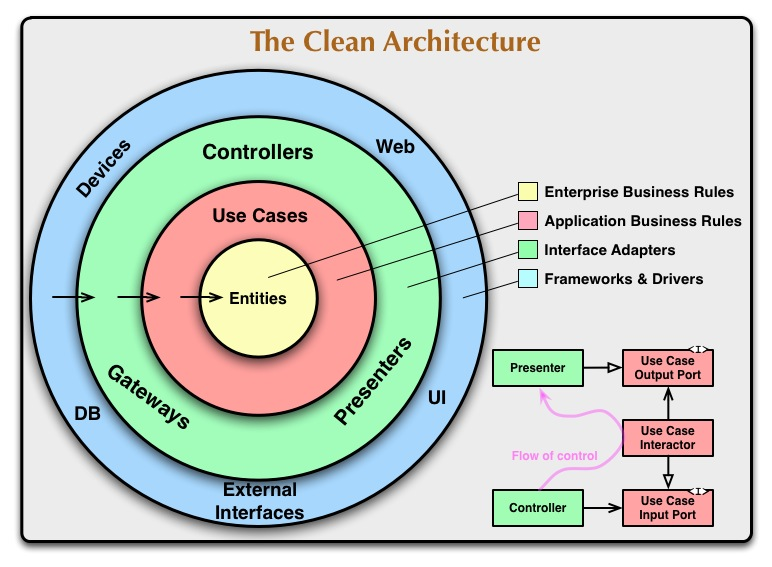
\includegraphics[width=0.8\columnwidth]{capitolo-6/architetture-confrontro/clean-architecture} 
    \caption{Diagramma dell'architettura Clean Architecture (da \cite{site:clean-architecture})}
\end{figure}